%
\chapter{Uvod v Ladijske elektronske naprave}
\label{intro_P} % Always give a unique label
% Po Darjan Jagnjić: SODOBNE NAPRAVE ZA PRAKTIČNO VODENJE VARNE POMORSKE NAVIGACIJE
 
Sodobne naprave in pripomočki za vodenje varne pomorske plovbe se samoumevno zelo razlikujejo od naprav pred digitalno revolucijo zaradi samodejnih zajemanj, preračunavanj in ergonomskih zaslonskih prikazov podatkov. Sodobni navigator je s sodobnimi napravami rešen precejšnjega bremena iskanj in preračunavanj. Digitalizirani podatki iz navigacijskih naprav se v predpisanih časovnih intervalih samodejno izrisujejo na zaslonu z elektronsko pomorsko karto in shranjujejo v pomnilne enote. 

Navigator, ki premišljeno uporablja iz podatkov pridelane informacije, poskrbi, da je dosežen varnostni vidik elektronskih naprav. Kljub stalni pomoči in celo nasvetom elektronskih naprav je vedno sposoben odgovoriti na osnovno vprašanje: \textit{Kaj se bo zgodilo z navigacijsko rešitvijo, če mi iz kateregakoli vzroka odpove ena naprava ali če odpove celoten elektronski sistem za vodenje varne navigacije?}


%http://www.glasnavigation.com/observations.html#.WOUYAccUzY4.linkedin
%Some of the basic essentials for safe navigation appear to be going unrecognized therefore uncorrected. These affect electronic navigation including ECS, ECDIS, and RADAR as well as conventional course and bearing applications. The alignment of the navigation equipment being installed parallel with the centerline of the vessel is paramount. Modern radars have the ability to adjust the heading alignment thru a firmware interface. Many times I’ve observed installations with the Radar Heading Marker offset by a couple of degrees. Proper alignment of the radar heading is essential for transiting narrow channels, and avoiding allisions / collisions, especially during periods of reduced visibility. Crews have become desensitized to the basics due to over dependence of AIS overlays on ECS and ECDIS displays. However, the same alignment issue is in play here, only worse. The gyro which provides the heading signal interfaced to all of the navigation electronics is in most cases askew, offset by a degree or more. The proper procedure starts with the installation of the foundation bracket for the gyro. The foundation bracket needs to be aligned with the centerline axis of the vessel, along with the slotted mounting holes on the base of the gyro allowing for finer adjustment of the housing. Then comes the Latitude compensator adjustment, the newer gyros handle this process internally with firmware thru a GPS input. The older units use either a potentiometer based adjustment or a mount based physical Latitude Corrector which slews the entire gyro housing on the foundation. The latter is found to be the one most misunderstood and set incorrectly.


\begin{figure}
	\centering
	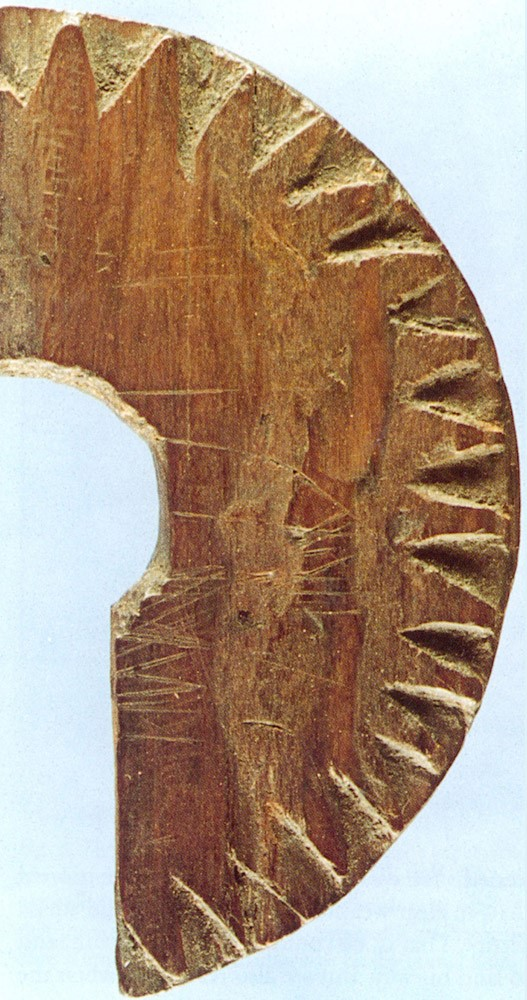
\includegraphics[height=5cm]{Predavanja/01_Uvod/figs/Sun_Compass_d.jpg}
	\hspace*{1.0cm}
	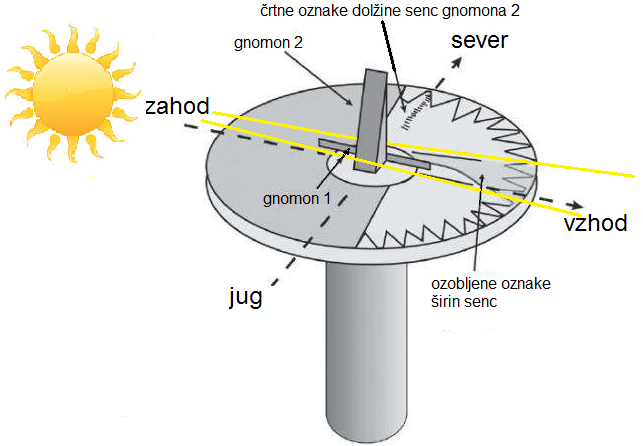
\includegraphics[height=5cm]{Predavanja/01_Uvod/figs/RekonstrukcijaVikingSunCompass_s.png}\\
	\vspace*{0.25cm}
	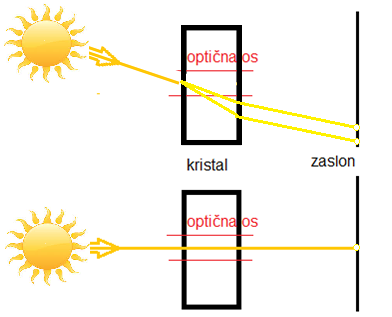
\includegraphics[height=5cm]{Predavanja/01_Uvod/figs/Kristal-SonceVInIzOPticneOsi_.png}
	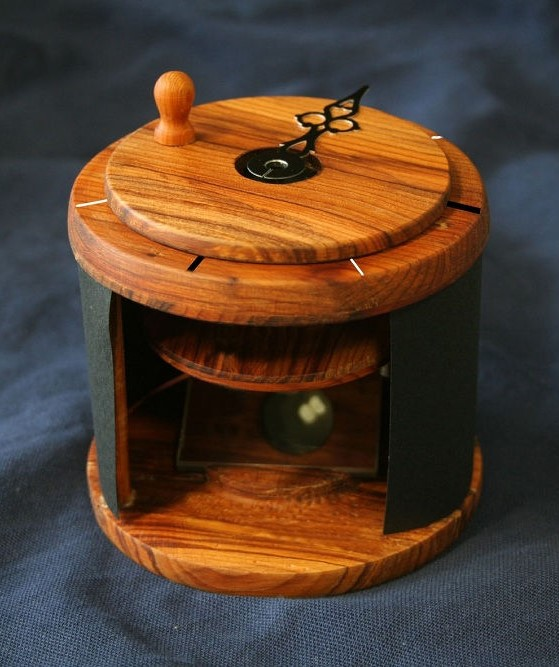
\includegraphics[height=5cm]{Predavanja/01_Uvod/figs/VikingSunstoneCompass.jpg}
	\caption{\textbf{Sončni kompasi} (zgoraj) Disk iz Uunartoka, Grenlandija, najden v samostanu iz 11. stoletja, naj bi predstavljal izsek sončnega kompasa Vikingov. Rekonstrukcija: \href{DOI: 10.1098/rspa.2016.0171}{\textit{Dénes Száz et al., Eötvös Loránd Tudományegyetem, Madžarska}} (spodaj) Ko so srednjeveški pomorščaki optično os prozornega dvolomnega monokristala kalcita z Islandije usmerili natančno v Sonce, so dobili na zaslonu namesto dveh pik le eno, s čimer so lahko določali smeri neba tudi v manj jasnih dneh. Rekonstrukcija: \href{http://www.livescience.com/16831-viking-sunstone-crystal-compass.html}{\textit{Guy Ropars, Université de Rennes, Francija.}}}
	%\href{http://spaceplace.nasa.gov/gps-pizza/en/}{\textit{GPS and the Quest for Pizza}}
	% KOMPAS Dénes Száz et al. North error estimation based on solar elevation errors in the third step of sky-polarimetric Viking navigation, Proceedings of the Royal Society A: Mathematical, Physical and Engineering Science (2016). DOI: 10.1098/rspa.2016.0171	Read more at: http://phys.org/news/2016-07-experimentation-vikings-sunstone.html#jCp
	% Balázs Bernáth, et al. "An alternative interpretation of the Viking sundial artifact: an instrument to determine latitude and local noon." Proceedings of The Royal Society A. DOI: 10.1098/rspa.2013.0021  Read more at: http://phys.org/news/2013-04-errors-viking-sun-compass-hint.html#jCp
	% KRISTAL http://www.sciencemag.org/news/2011/11/viking-sunstone-revealed
	% http://myphysicshelp.weebly.com/double-refraction.html
	% http://www.livescience.com/16831-viking-sunstone-crystal-compass.html
	% Orientation with a Viking sun-compass, a shadow-stick, and two calcite sunstones under various weather conditions Balázs Bernáth, Miklós Blahó, Ádám Egri, András Barta, György Kriska, and Gábor Horváth Applied Optics Vol. 52, Issue 25, pp. 6185-6194 (2013) •doi: 10.1364/AO.52.006185
	\label{fig:SoncniKompas}       % Give a unique label
\end{figure}



Poglavja v tej knjigi so namenjena bodočim pomorščakom, da z njimi dobite čim boljši vpogled v celoto vodenja varne plovbe v vseh okoliščinah. Poglavja vsebujejo spoznavanje osnov klasičnih, toda vedno uporabnih naprav in sredstev za vodenje načrtovane plovbe v vseh pogojih, tudi takrat, ko na sodobno opremljenih ladjah odpovedo prej omenjene sodobne elektronske naprave in sredstva za vodenje navigacije v združenih (integriranih) navigacijskih sistemih. V nadaljevanju boste spoznali najsodobnejše naprave in sredstva za vodenje elektronske navigacije in njihovo zanesljivost v okolju, ki jih obdaja.


\section{Osnovna načela in pojmi}
\label{sec:OsnNacela}

Določanje položaja in hitrosti\footnote{hitrost je vektor, torej poleg velikosti določamo tudi smer gibanja} premikajočih se objektov glede na znano referenčno točko se v strokovni literaturi imenuje \textbf{navigacijska znanost}. Ročno ali samodejno načrtovanje in vzdrževanje kurza od ene točke do druge, izogibajoč se oviram in trčenjem, pa se v literaturi pojavlja kot \textbf{umetnost navigacije}, kar v vsakdanjem jeziku imenujemo ali vožnja ali pilotiranje ali krmarjenje, odvisno od vrste prevoznega sredstva. 

Pričujoča knjiga je prvenstveno namenjena razlagi ozadja umetnosti navigacije, zaradi poglobljenosti pristopa bomo omenili tudi nekaj elementov navigacijske znanosti.

\subsection{Osnovni strokovni izrazi v pomorski navigaciji in komunikaciji}
\label{SubSec:OsnStrokIzrNav}

Med navigacijo je \textit{uporabnik}, ki je lahko ali oseba ali računalniški program, del objekta, ki se mu določa položaj. Delom navigacijskega sistema, ki mu določamo položaj, rečemo \textbf{uporabniška oprema}. 

Rezultat navigacije imenujemo \textbf{navigacijska rešitev}, ki vključuje položaj in hitrost objekta, nekateri navigacijski sistemi določajo tudi smer gibanja (v pomorstvu kot med geografskim severom in smerjo plovbe imenujemo \textit{kurz}). Predvsem inercijski sistemi določajo tudi pospešek in kotno hitrost. V navigaciji pomorske plovbe zadostujeta obe vodoravni komponenti položaja in hitrosti, v podmorniški navigaciji je potrebno poznati tudi navpično komponento.

Izraza \textbf{lokacija} in \textbf{položaj} imata različen pomen, čeprav ju v praksi večkrat med seboj zamenjujemo. Oba pojma podajata navigacijsko rešitev uporabnika, razlika je v velikosti območja te rešitve. Določanje lokacije (lociranje) v praksi pomeni poimenovanje območja cilja (npr. pristanišče ali oznako priveza), še posebno, ko je \textit{navigator-umetnik} sorazmerno blizu cilja. Določanje položaja (pozicioniranje) pa znanstvenik definira z območjem okoli navigacijske rešitve v obliki koordinat izbranega koordinatnega sistema. Geodet zahteva za rezultate svojega dela pod1cm točnost, karte hidrografov morajo zagotavljati pod10cm točnost. Za navigacijo med plovbo pa predpisi IMO praktičnemu navigatorju narekujejo uporabo naprav, ki v vodoravni ravnini s 95 odstotno verjetnostjo zagotavljajo pod10m točnost, med manevriranjem v pristanišču pa pod2,5m.

% IMO, podatki 2013
%http://www.ignss.org/LinkClick.aspx?fileticket=b%2F3x6KEaFS4%3D&tabid=56

Aktivna in pasivna orientacijska znamenja (angl. landmark) na znanih položajih, na primer svetilniki ali odsevniki (ang. reflectors), ki so nameščena samo zaradi navigacije, se imenujejo \textbf{navigacijski pripomočki} (ang. Aids to navigation, AtoN). K navigacijskim pripomočkom štejemo tudi satelite GNSS, saj mora za določitev lastnega položaja sprejemnik GNSS zelo točno poznati položaj satelita v trenutku, ko je oddal določen signal.


%SLIKA klasični (fotografiram Darjanov log na SŠ) in elektromagnetni log
%klasični log: http://www.pbenyon.plus.com/B_S_M/Log_Line.html
%ladijske razbitine: Peter Reaveley (22 June 2010). "Navigation and Logbooks in the Age of Sail". United States Naval Academy. Retrieved 18 February 2015. https://www.usna.edu/Users/oceano/pguth/website/shipwrecks/logbooks_lesson/logbooks_lesson.htm 

\begin{figure}
	\centering
	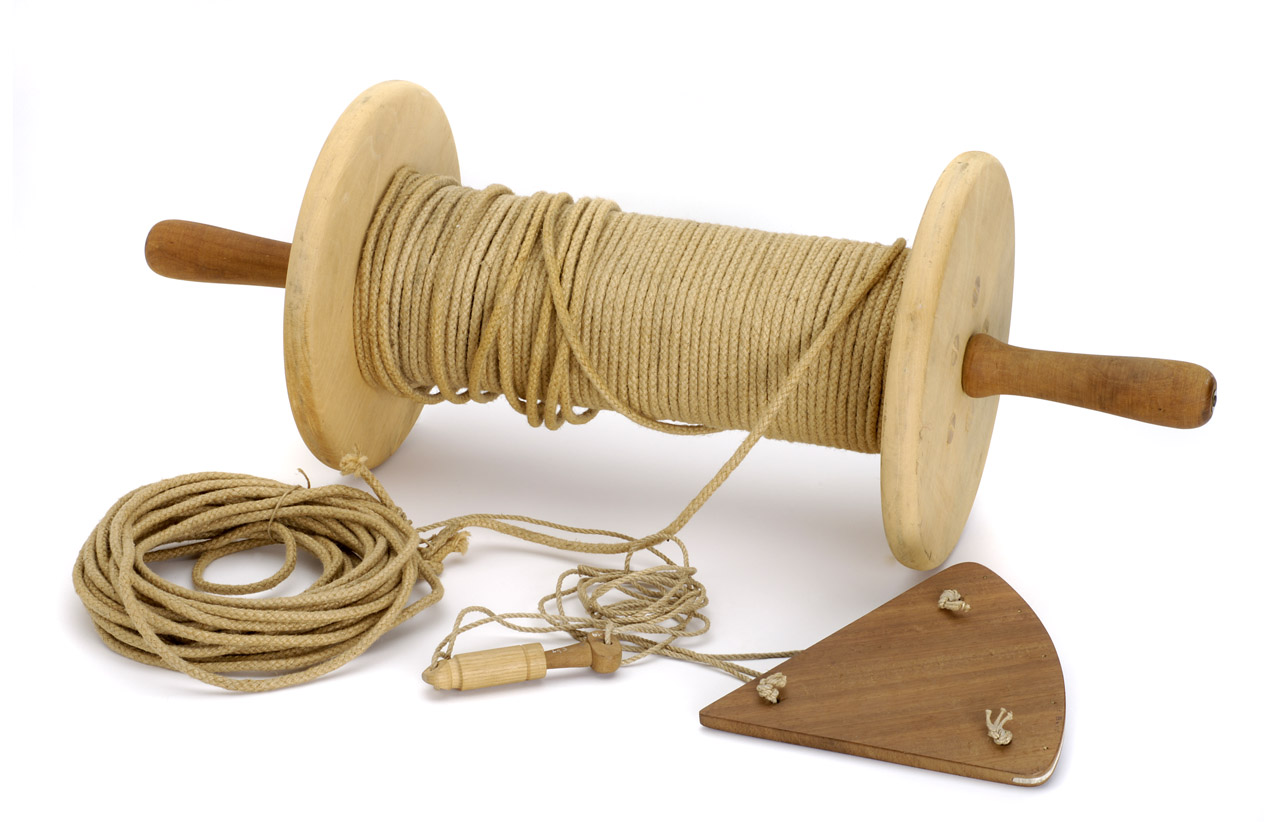
\includegraphics[height=5cm]{Predavanja/01_Uvod/figs/LeseniLog.jpg}
	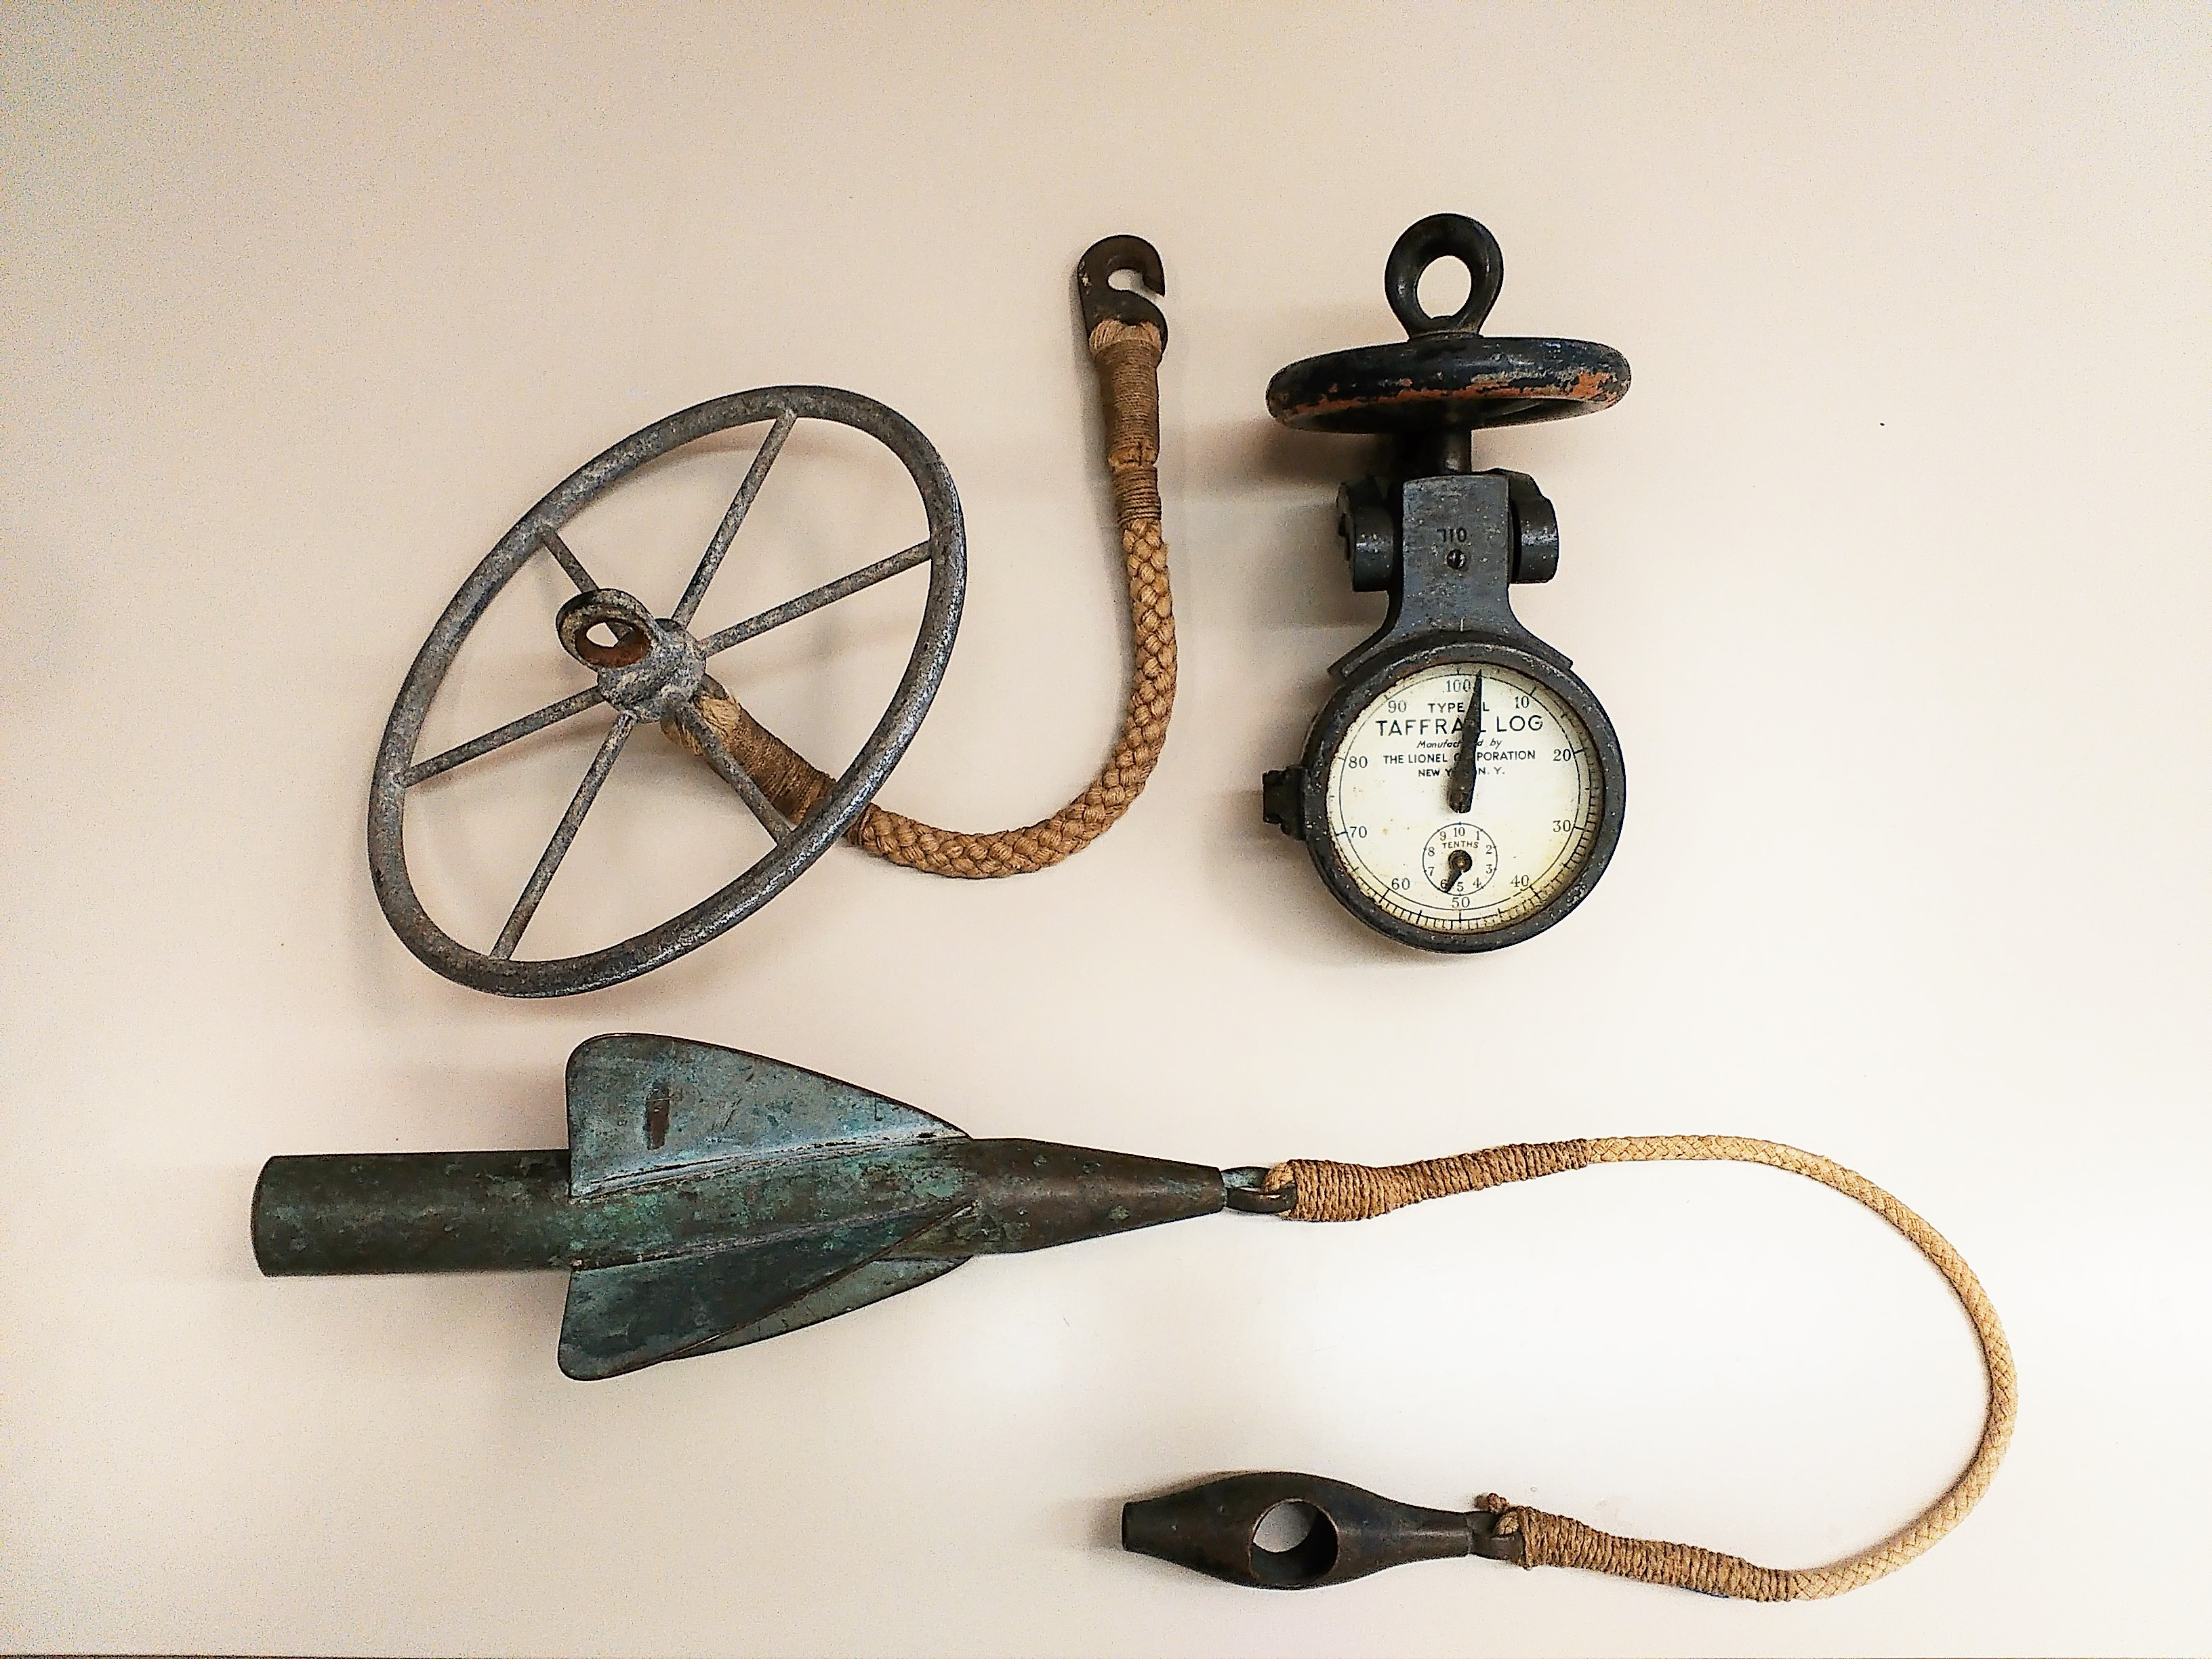
\includegraphics[height=5cm]{Predavanja/01_Uvod/figs/BronastiLog_2016-11-25_k.jpg} %BronastiLog_meiVWri9CXBiW03hPmRrppQ.jpg}
	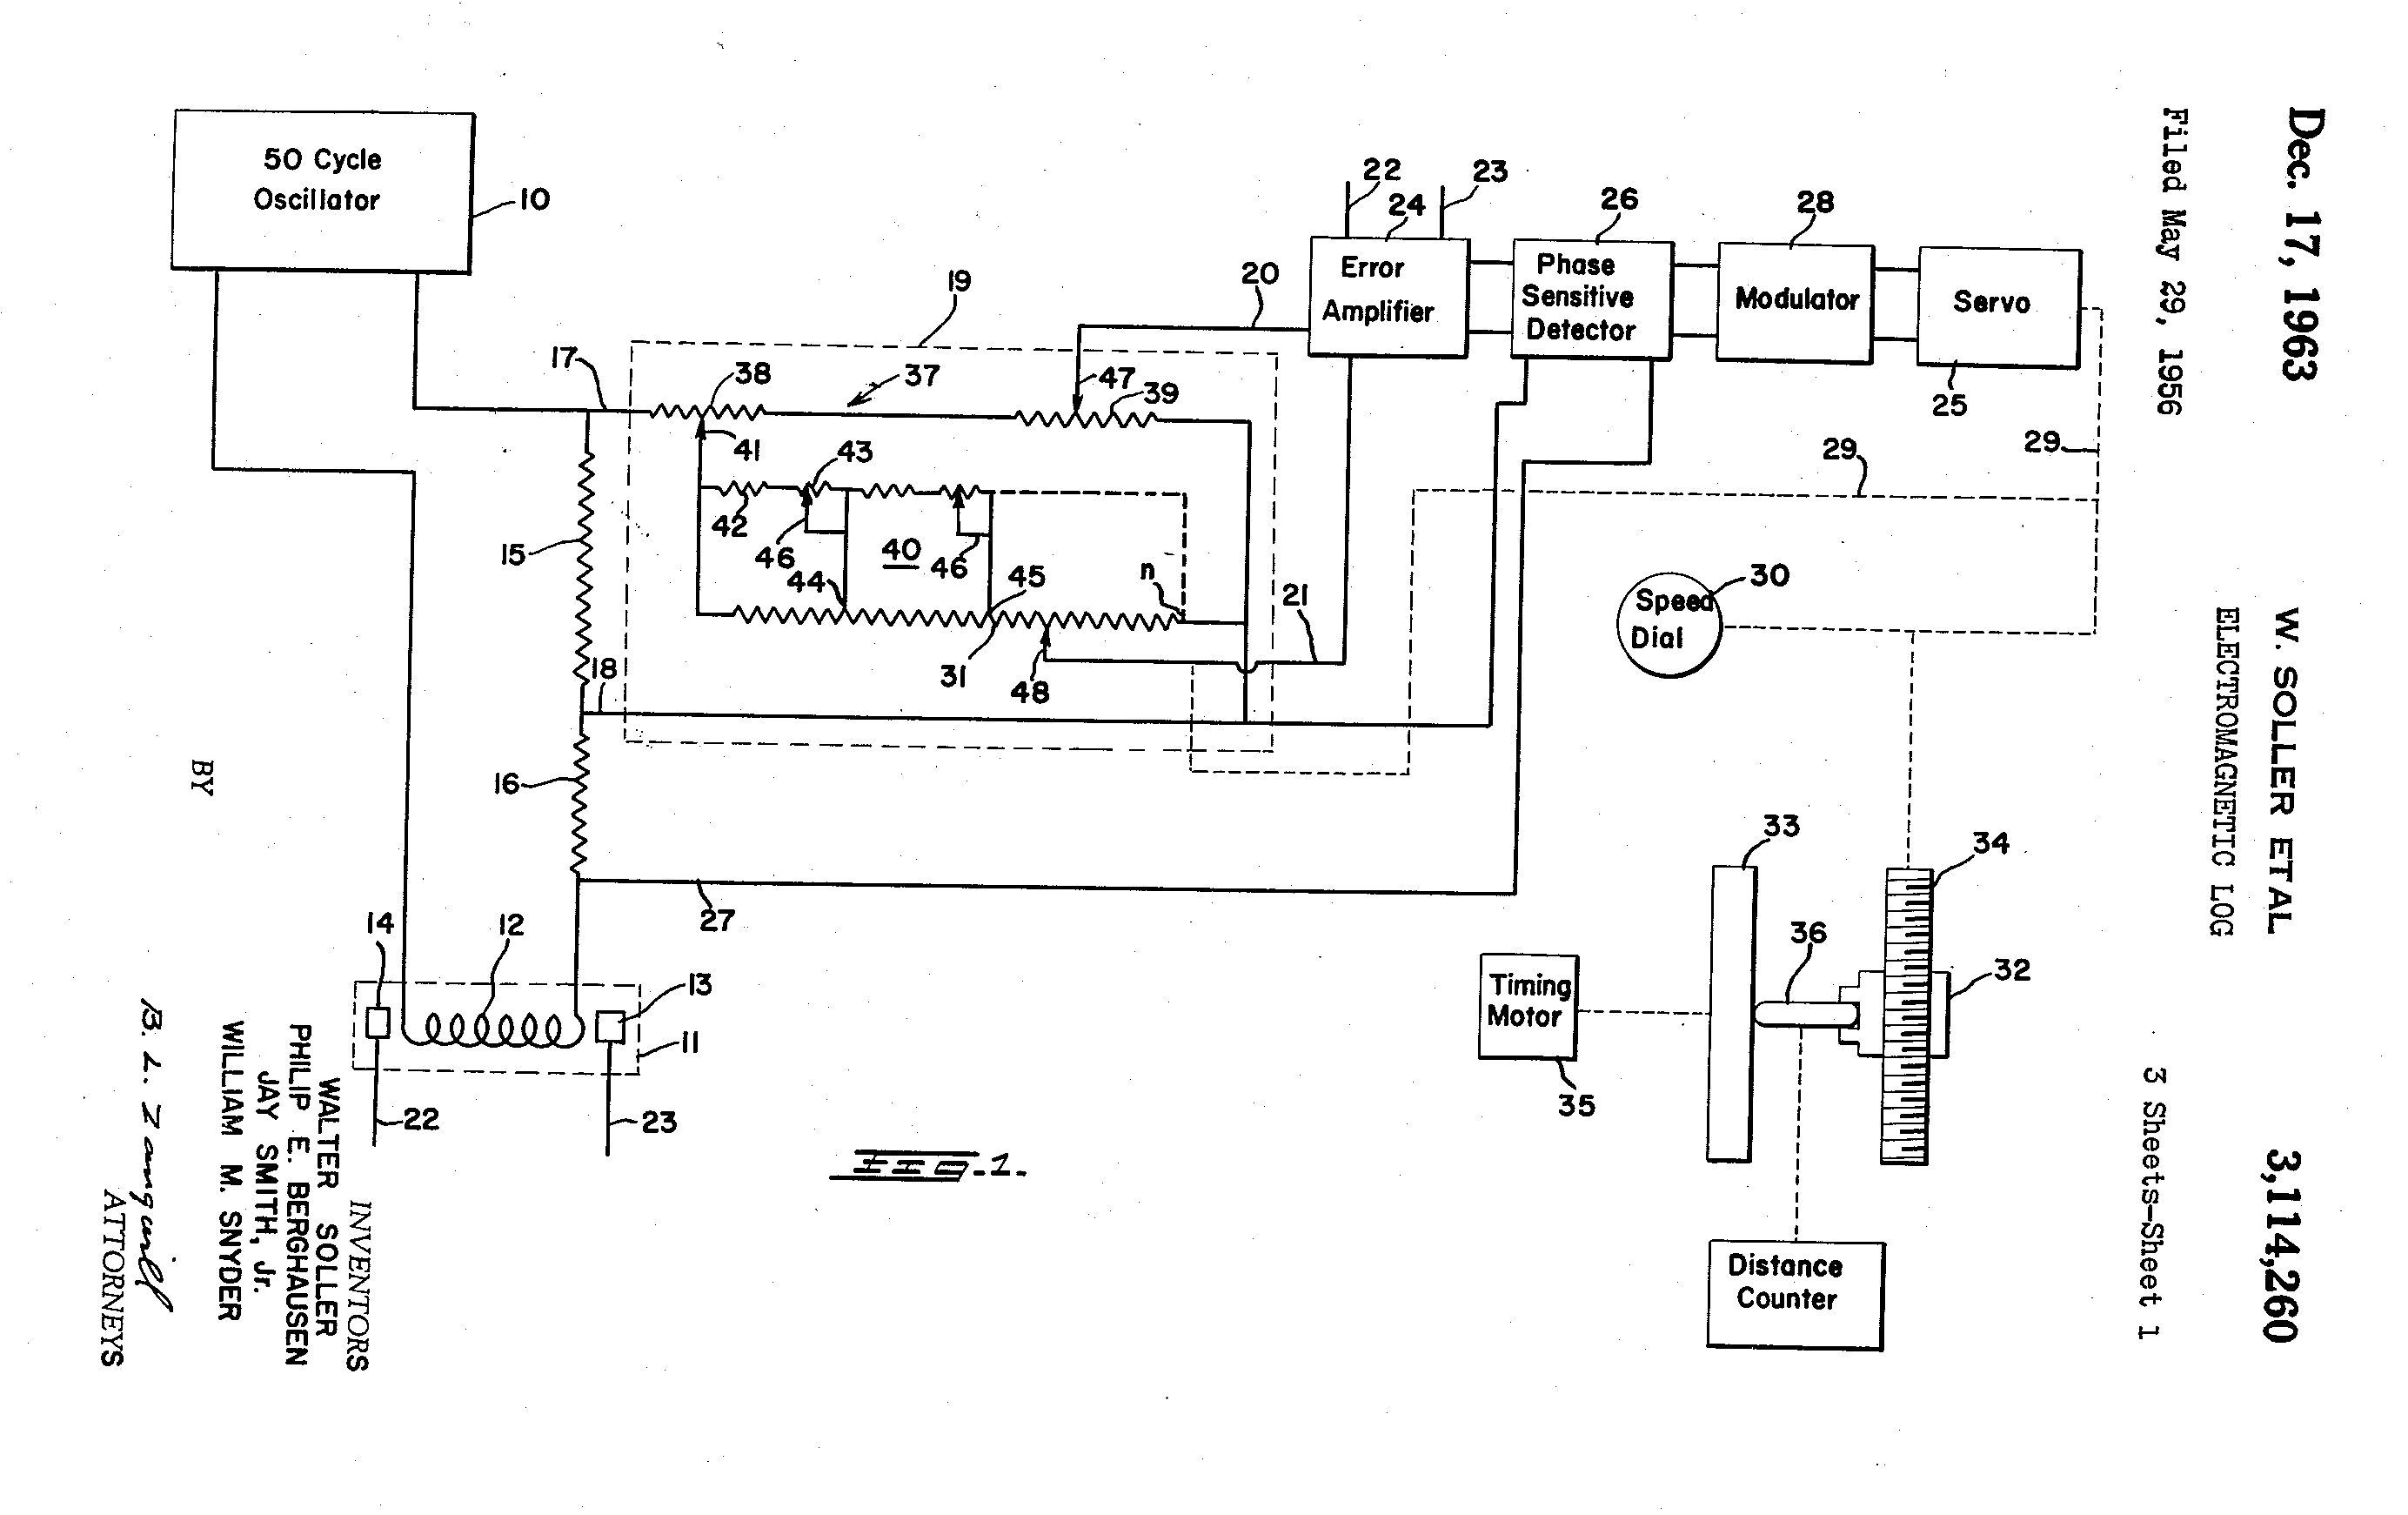
\includegraphics[height=5cm]{Predavanja/01_Uvod/figs/US3114260-0_EM-Log.png}
	\caption{\textbf{Merilniki hitrosti - logi} (zgoraj) Leseni (ang. chip) log, pripisan domnevnemu iznajditelju Bartolomeu Crescêncio, Portugalska, 15./16. stoletje. Dokumentirani vir: \href{http://quod.lib.umich.edu/cgi/t/text/text-idx?c=eebo;idno=A16510.0001.001}{\textit{William Bourne, A Regiment For the Sea, pogl. 14, 1574}} (sredina) V 19. stoletju je leseni log nadomestil bronasti (ang. patent, taffrail) log z vrtečim se vijakom, arhiv GEPŠ, Portorož. (spodaj) Elektromagnetni log s sabljičastim tipalom nima več premikajočih se delov, sicer ni tako točen kot Dopplerjev log, a omogoča digitalni zapis. Izumitelji: \href{https://www.google.com/patents/US3114260}{\textit{Philip E. Berghausen, Jay Junior Smith, William M. Snyder, Walter Soller, 1963, ZDA}}}
	%\href{http://spaceplace.nasa.gov/gps-pizza/en/}{\textit{GPS and the Quest for Pizza}}
	\label{fig:Logi}       % Give a unique label
\end{figure}

% Now don’t be scared: These famous T-shirt equations, written in a mathematical language that James Clerk Maxwell partly had to invent, defined the properties of the second Quantum Field: Electromagnetism.
%They read like a foreign language, but learning about them is not all that difficult once you know what the symbols mean. But they are clearly meant for people who fill blackboards full of this stuff. There are many ways of writing these equations, and however they are written, they say something pretty remarkable. The second equation for example, says there can’t be magnetic monopoles, even though the equation above it defines electric monopoles, or the force caused by static charges. Remarkably, the fourth equation is a wave equations used to calculate the speed of electromagnetic waves in a vacuum; “c” which works out to be 2.99792458 x 10E8 meters per second (present day, agreed-upon number).
%Maxwell calculated “c” as a function of two other physical constants, the Permittivity and Permeability of a vacuum, values that are not hard to measure. So Maxwell’s “c,” calculated in 1861–2 is perfect and absolute depending only on the accuracy of the other constants. The equation describes the electromagnetic nature of the vacuum…nothing else! To believe anything can go faster than light is to believe that there is something that has a Permittivity and Permeability less than vacuum. So in a very fundamental way, you can’t get a more accurate measurement for “c” or for any electromagnetic phenomena in a vacuum. Remember, Maxwell was talking only about the characteristic of the electromagnetic field.
%So the velocity of light was known to ridiculous precision half-a-century before Einstein. Amazing. Both Einstein and Feynman considered this the most important advance to come along in centuries. 

Sodobna pomorska komunikacija ni izvedljiva brez (\href{http://missionscience.nasa.gov/ems/05_radiowaves.html}{elektromagnetnih valov}), ki jih v vsakdanjem jeziku običajno imenujemo radijski valovi, v resnici pa predstavljajo množico valovanj, ki nastajajo zaradi verižnih sprememb električnega in magnetnega polja. V tej praktično neskončni verigi je prvo polje vzrok za nastanek drugega, ki je vzrok za nastanek prvega, ki je spet vzrok za nastanek drugega, ... Do katere razdalje od izvora valovanja nas ta veriga zanima, je odvisno od občutljivosti sprejemnika in njegove sposobnosti obdelave sprejetega signala.

Vse vrste elektromagnetnih valov se razširjajo s \textit{hitrostjo svetlobe}. Ko dejansko izmerimo kolikšno pot prepotuje svetloba v eni sekundi, dobimo v okviru naše merilne natančnosti rezultat, podoben rezultatu, ki ga dobimo iz dveh konstant vakuuma: njegove permeabilnosti in dielektričnosti. Hitrost svetlobe in tudi vseh elektromagnetnih valovanj v vakuumu je namreč $c_0 = 2,99792458 10^8m/s$. Od 1983 naprej je hitrost svetlobe v vakuumu $c_0$ privzeta kot konstanta.

Komunikacija ladje s kopenskimi postajami je možna zaradi razširjanja radijskih valov, ki glede na lastno frekvenco izberejo eno od poti (glej sliko \ref{fig:PotiRazsirjanjaEmv}): ali sledijo zemeljski povšini (kopenski val) ali se širijo v približno ravni črti (kvazioptočni val) ali pa se zaradi postopnega loma v ionosferi vrnejo nazaj na Zemljo (prostorski val). 

\begin{figure}
	\centering
	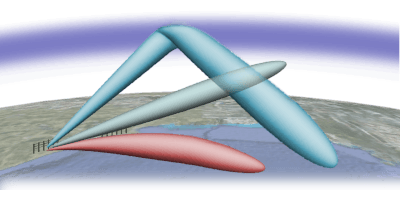
\includegraphics[width=\textwidth]{Predavanja/01_Uvod/figs/PotiRazsirjenjaValov.png}
	\caption{Troje poti razširjanja elektromagnetnih valov. (vir: radartutorial.eu)}
	\label{fig:PotiRazsirjanjaEmv}       
\end{figure}


Dokler je sprejemna radijska postaja (\textbf{sprejemnik}) v neposrednem dosegu oddajne postaje (\textbf{oddajnika}), rečemo, da je sprejemnik znotraj radijskega horizonta oddajnika. Na območje \textit{slišnosti} oddajnika oz. na razdaljo do radijskega horizonta vplivata frekvenca radijskih valov in ukrivljanje poti razširjanja oz. lom (ang. refraction) v najnižji, troposferski plasti atmosfere. Standardna atmosfera pomeni na srednji višini morja zračni tlak $1013,25hPa$, ki ob dvigovanju pada z $11,8hPa/100m$, hitrost zvoka $340,3 m/s$ temperaturo $15^{\circ}C$, ki z višino upada za $6,5^{\circ}C/1000m$  in gostoto zraka $1,255kg/m^3$ ter z relativno vlažnostjo $60\%$, ki se z višino ne spreminja. Parameter relativne vlažnosti je zelo teoretičen, vendar vsako odstopanje od omenjene vrednosti pomembno vpliva na lomni količnik in s tem na domet radijskih zvez in radarjev v pomorski praksi. 

%https://ntrs.nasa.gov/archive/nasa/casi.ntrs.nasa.gov/19770009539.pdf
%https://en.wikipedia.org/wiki/International_Standard_Atmosphere
%http://www-mdp.eng.cam.ac.uk/web/library/enginfo/aerothermal_dvd_only/aero/atmos/atmos.html
%http://www-mdp.eng.cam.ac.uk/web/library/enginfo/aerothermal_dvd_only/aero/atmos/stdatm.html

Dimnik ladje se dviga $h_{dimn}$ nad gladino. Obzorje opazujemo na dva načina: a) \textit{optično} z daljnogledom in b) \textit{radijsko} z radarjem. Nastavitve radarja predvidevajo, da se njegovi valovi razširjajo v standardni atmosferi oz., da nastaja standardni lom radijskih valov. Ladijsko opločje je na višini $h_{oplo"c}$, ki sega do palube in zanesljivo odseva glavnino valov iz radarske antene. Na zaslonu radarja v pogojih standardne atmosfere opazimo opločje že precej prej, kot z očesom opazimo vrh dimnika iste ladje. Primerjava optičnega horizonta $D_{opt}$ (enačba \ref{eq.D.opt}) in radijskega horizonta $D_{rad}$ (enačba \ref{eq.D.rad}) vzbuja pomislek, da se polmer Zemlje $R_Z$, ki znaša na ekvatorju $6370km$, kar prilagaja radijskim valovom:

\begin{equation}\label{eq.D.opt}
D_{opt}=\sqrt{2h_{dimn}R_Z}
\end{equation}

\begin{equation}\label{eq.D.rad}
D_{rad}=\sqrt{2h_{oplo"c}R_{ekviv}}.
\end{equation}

Ko primerjamo enačbi vidimo, da je $R_{ekviv} < R_Z$ manjši zaradi razširjanja valov skozi suhe hladne plasti nad toplejšimi morji in zaradi naraščanja vlažnosti z višino (ang. sub-refraction), zaradi česar se pot valov ukrivlja od gladine navzgor in je $D_{rad} < D_{opt}$ (glej sliko \ref{fig:LomiAtmosfera}). Če pa temperatura narašča z višino, vlažnost pa naglo upada, ko npr. hladnejše gladine morij obliva toplejši zrak, nastanejo pogoji super-loma (ang. super-refraction), kar poveča horizont in zaradi $R_{ekviv} > R_Z$ postane $D_{rad} > D_{opt}$, pojavljajo se moteči odboji (ang. clutter) na površini. Zaradi močnega temperaturnega obrata (hladen zrak nad gladino, nad njim skokovito suh topel zrak) lahko nastanejo pogoji (ang. ducting), ko je $R_{ekviv} >> R_Z$, ker se pot radijskega vala ujame med meji temperaturno invertiranega nadvodnega pasu, zaradi česar radarska slika izrisuje nepričakovane odseve daljnih pojavov, radijski sprejemnik pa sprejema signale iz zelo oddaljenih krajev. 

%http://www.splashmaritime.com.au/Marops/data/text/Radartex/Radartex.htm

\begin{figure}
	\centering
	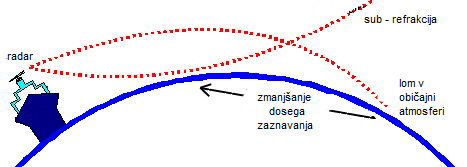
\includegraphics[width=\textwidth]{Predavanja/01_Uvod/figs/Subrefraction.png}
	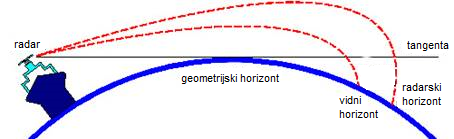
\includegraphics[width=\textwidth]{Predavanja/01_Uvod/figs/OpticniRadarskiHorizont.png}	
	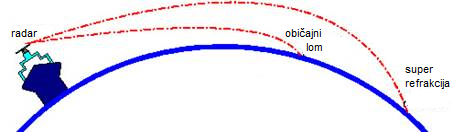
\includegraphics[width=\textwidth]{Predavanja/01_Uvod/figs/RefractionSuperrefraction.png}
	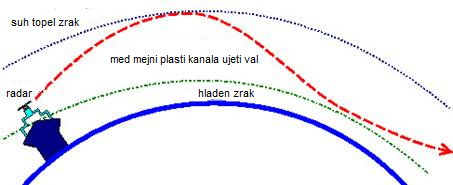
\includegraphics[width=\textwidth]{Predavanja/01_Uvod/figs/Valovod.png}	
	\caption{Od zgoraj navzdol: naraščanje dosegov elektromagnetnih valov zaradi različnih stanj atmosfere. (splashmaritime.com.au)}
	\label{fig:LomiAtmosfera}       
\end{figure}

%ANTENE: Maritime Antennas Market: By Antenna Type (VHF, AIS, WI-FI, Cellular, SATCOM, Others) By Frequency (VHF, HF, MF, SHF, EHF); By End-User (Fishing, Merchant, Offshore, Others) & By Geography

Oblika profila temperatur nad morsko gladino torej odloča ali bo doseg radijskih valov krajši ali daljši kot pri standardni relativni vlažnosti s prostim očesom. 

%https://en.wikipedia.org/wiki/Anomalous_propagation 
%This type of false return is relatively easy to spot on a time loop if it is due to night cooling or marine inversion as one sees very strong echoes developing over an area, spreading in size laterally, not moving but varying greatly in intensity with time. After sunrise, the inversion disappears gradually and the area diminishes correspondingly. Inversion of temperature exists too ahead of warm fronts, and around thunderstorms' cold pool. Since precipitation exists in those circumstances, the abnormal propagation echoes are then mixed with real rain and/or targets of interest, which make them more difficult to separate.
%Doppler radars and Pulse-Doppler radars are extracting the velocities of the targets. Since AP comes from stable targets, it is possible to subtract the reflectivity data having a null speed and clean the radar images. Ground, sea clutter and the energy spike from the sun setting can be distinguished the same way but not other artifacts.[3][4] This method is used in most modern radars, including air traffic control and weather radars.

\subsection{Tehnike določanja položaja}
\label{SubSec:TehnDolPoloz}

Elektronske naprave za določanje položaja omogočajo določanje položaja v izbranem koordinatnem sistemu oz. glede na dano izhodišče. Če je izhodišče središče zemeljskega koordinatnega sestava, določamo s takšnimi napravami \textit{absolutni položaj} (kot npr. s sprejemnikom GNSS), če je izhodišče položaj antene na plovilu (kot npr. pri navigacijskem radarju), določamo z njimi \textit{relativni položaj}. 

Načine določanja položaja motrimo z vsaj s tremi pogledi, v vsakem pogledu se pojavljata po dva razreda. 

\textbf{1. pogled} Pomorski navigatorji iz razumljivih razlogov potrebujejo podatke o položaju takoj po opravljeni meritvi, med daljšim manevriranjem celo neprekinjeno, na drugi strani pa so geodeti ali hidrografi (zaenkrat še) zadovoljni, če podatke dobijo šele čez nekaj ur ali celo čez nekaj dni po opravljenih meritvah. Če se nam torej zdi pomembna \textit{hitrost pridobitve podatka o položaju}, načine delimo na dva razreda: tehnike sprotnega pridobivanja rezultata položaja (v realnem času) in tehnike pridobivanja z naknadno obdelavo (ang. post processing).      

\textbf{2. pogled} Med plovbo (\textit{navigacijo}) se plovilo giblje, geodeti pa na terenu večinoma merijo položaje mirujočih objektov. Glede na gibanje objekta, ki mu določamo položaj, ločimo dva razreda: če se objekt med meritvijo giblje, se način določanja položaja imenuje kinematična tehnika, če pa se ne giblje, način imenujemo statična tehnika.

\textbf{3. pogled} Na določanje položaja lahko gledamo praktično: ločimo načine določanja lastnega položaja (ang. self-positioning) in tujega položaja (ang. remote positioning).

V praksi seveda delo s podatki konkretnih elektronskih naprav uvrščamo hkrati v več razredov. Na primer tehnike pridobivanja podatkov iz navigacijskega radarja spadajo v razred kinematičnih sprotnih tehnik določanja tujega \textit{relativnega} položaja.

\subsection{Tehnike določanja smeri}
\label{SubSec:TehnDolS}

\section{Razdelitev dela Predavanja}
\label{sec:Uvd_RazdPred}

%here is a list of ship electronic devices you should learn about:
%
%- ship course deternimation using compass (magnetic, gyroscopic, fibre optic, electromagnetic)
%- relative postioning of other objects: Radar
%- navigation using depth-sounder
%- terrestrial positioning using radio waves from platforms on Earth: e-Loran
%- terrestrial positioning using radio waves from platforma in space: Global Navigation Satellite Systems and Satellite based Augmentation Systems (EGNOS)
%- Electronic Chart and Display Information System
%- Global Maritime Distress and Safety System basics: Maritime Mobile Services (capabilities of every SOLAS ship), transmitter and receiver basics (modulation), basics of propagation of electromagnetic waves (3 ways of paths, refraction, radio horizon, attenuation), sources of electrical energy on ship, antenae.   
% When you are ready to explain their aims, their regular use, errors which may occur during exploatation, and handling those errors just let me know you are ready for oral examination.
%
% Use the any available paper or digital source, I recommend digital library - ask our librarians. If you use wikipedia explanations take them only for the start, and then deepen your understanding with maritime (IMO) sources. 

Zaradi praktičnosti so navigacijske naprave v tej knjigi razdeljene na naprave za določanje lastnega in tujega položaja. Začetki določanja lastnega položaja segajo v čase prvih iskalcev boljših pogojev za življenje in bogatejših naravnih virov. Prvim raziskovalcem neznanega sveta je poznavanje tehnik določanja položaja povečevalo možnost preživetja s primernim načrtovanjem porabe zalog in povratka v znana okolja. Določanje tujega položaja, na primer razporeditve položajev sovražnih bojevnikov, se je najprej razvilo predvsem iz potreb po lastni varnosti.

V poglavju \textit{Kompasno določanje smeri} je zbran pregled dejstev, zakonov in načinov, ki omogočajo določanje smeri pogleda oz. smeri plovbe (kurza). Ker kompasi med plovbo omogočajo izurjenim navigatorjem tudi določanje položaja, poglavje sega tudi na področje določanje položaja. Poglavje \textit{Elektronsko določanje položaja} zajema dejstva, ki jih mora pomorščak poznati, da lahko razume tehnike določanja lastnega položaja s pomočjo pomorskih kart in v poglavju opisanih elektronskih naprav. Sledi poglavje \textit{Zemeljsko določanje lastnega položaja}, v katerem so opisane metode za določanje lastnega položaja s pomočjo referenčnih točk na Zemlji. Logično nadaljevanje je poglavje \textit{Satelitsko določanje lastnega položaja} z opisi sistemov z umetnimi in naravnimi referenčnimi točkami v vesolju. V poglavju \textit{Določanje tujega položaja} smo se osredotočili na naprave za določanje položaja in hitrosti okoliškim objektom. \textit{Predstavitev omrežij in posebnosti protokola NMEA2000}, standardiziranega kot IEC 61162-3, zajema kratek opis razvoja, zgradbo in opis delovanja standardnih ladijskih omrežij za zajem in izmenjavo podatkov med ladijskimi napravami. Posebno poglavje \textit{Povzetek napak in njihovo odpravljanje} daje pregled nad pomembnejšimi napakami naprav in načini odpravljanja njihovih posledic. Povzetek glavnih točk doslej omenjenih naprav je zbran v poglavju \textit{Povzetek sodobnih navigacijskih sistemov}, v katerega so vključeni tudi zasnove elektronskega kartiranja in uporaba združenih (integriranih) sistemov. Ker med elektronske naprave poleg navigacijskih spadajo tudi komunikacijske, je njihovemu opisu in delovanju posvečeno poglavje \textit{Pregled komunikacijskih naprav in GMDSS}. Doseganje cilja plovbe, ki ga predvidi poveljnik plovila, in ga omogoča optimalno delovanje ladijskih strojev, vodenimi z inženiri stroja, povezujejo samodejne naprave, opisane v poglavju \textit{Sodobno krmarjenje ladje}.      

\vspace{1cm}
V pomoč pri študiju virov v angleškem jeziku vam je slovar v poglavju \ref{slovar}. 

%\begin{equation}
%\vec{a}\times\vec{b}=\vec{c}
%\end{equation}

 

%\cite{monograph}.

%
%
%
% Problems or Exercises should be sorted chapterwise
\section*{Vprašanja v razmislek in poglobitev}
\addcontentsline{toc}{section}{Vprašanja}
%
% Use the following environment.
% Don't forget to label each problem;
% the label is needed for the solutions' environment
\begin{prob}
\label{prob1}
Kakšne hitrosti so dosegale ladje v primerih, ki jih v izvirnem angleškem opisuje William Bourne? \textit{In like manner they have either a minute of an hour glass, or else a known part of an hour by some number of words, or such other like, so that the line being were out and stopped just with that time that the glass is out, or the number of words spoken, which done, they hale in the log or piece of wood again, and look how many fathom the ship has gone in that time: that being known,what part of a league should it be, they multiple the number of fathomes, by the portion of time or part of an hour. Whereby you may know just how many leagues and parts of a league the ship went in an hour. etc., W. Bourne, 1574} An English league contains 250 fathomes (imperial: 1,85324m; US: 1,8228m). A Spanish or Portugues league doth contains 2857 fathomes. etc.
\end{prob}

\begin{prob}
\label{prob2}
Kaj vse vpliva na določanje hitrosti plovila s pomočjo lesenega polena (loga) in peščene ure? \textit{Z lesenim polenom so pomorščaki hitrost plovila določali približno. V rezultatu meritve so ostali neznani vplivi valovanja morja oz. kakovost stika loga s površino, vpliv morskih tokov, elastičnost vrvi, nenatančnost merjenja časa zaradi nihanja temperature, relativne vlažnosti in valovanja morja, ki je vplivalo na enakomernost padanja peska v uri.} 

Ali bi takšne napake imenovali sistematske ali naključne?
\end{prob}

\begin{prob}
	\label{prob3}
	Poišči vrednosti permeabilnosti in dielektričnosti vakuuma in iz njiju izračunaj hitrost svetlobe v vakuumu? 
\end{prob}


%
